\documentclass[a4paper, twocolumn, oneside]{article}

\usepackage{xstring}
\usepackage{xparse}
\usepackage{blindtext}
\usepackage{amsfonts}
\usepackage{amsmath}
\usepackage{amssymb}
\usepackage{tikz}
\usepackage{algorithm}
\usepackage{algpseudocode}
\usepackage[backend=bibtex]{biblatex}

\usepackage[barriers=false]{acro}
\NewDocumentCommand\acrodef{mO{#1}mG{}}{\DeclareAcronym{#1}{short={#2}, long={#3}, #4}}
\NewDocumentCommand\acused{m}{\acuse{#1}}
\usepackage[hidelinks]{hyperref}
\usepackage[capitalise]{cleveref}
\crefname{section}{section}{sections}
\crefname{figure}{figure}{figures}
\crefname{table}{table}{tables}
\crefname{equation}{equation}{equations}
\crefname{algorithm}{algorithm}{algorithms}
\Crefname{section}{Section}{Sections}
\Crefname{figure}{Figure}{Figures}
\Crefname{table}{Table}{Tables}
\Crefname{equation}{Equation}{Equations}
\Crefname{listing}{Listing}{Listings}
\crefname{algorithm}{Algorithm}{Algorithms}
\def\figname{\csname cref@figure@name\endcsname\xspace}
\def\tabname{\csname cref@table@name\endcsname\xspace}
\def\secname{\csname cref@section@name\endcsname\xspace}
\def\eqname{\csname cref@equation@name\endcsname\xspace}
\def\eqpname{\csname cref@equation@name@plural\endcsname\xspace}
\def\eqname{\csname cref@listing@name\endcsname\xspace}
\def\eqname{\csname cref@listing@name@plural\endcsname\xspace}

\acrodef{CMKP}{Clustered Multidimensional Knapsack Problem}
\acrodef{ILP}{Integer Linear Problem}
\acrodef{MKP}{Multidimensional Knapsak Problem}

\title{The \ac{CMKP}}
\author{E.Brambilla, M.Cherubini, S.Fontana, C.Metelli, J.Tedeschi}
\date{\today}
\addbibresource{bibliography.bib}

\begin{document}
\twocolumn[
  \begin{@twocolumnfalse}
    \maketitle
    \begin{abstract}
      This project aims to provide an efficient heuristic method to approach the \ac{CMKP} capable of producing good feasible solutions in a limited-time environment. This project will be evaluated against the solutions of benchmark instances found by the Gurobi\cite{gurobi} solver, The goal of this project is to deonstrate the above-mentioned heuristic can deliver close -- or better -- solutions to the plain solver results in a reduced amount of time.
    \end{abstract}
    \vspace{5mm}
  \end{@twocolumnfalse}
]

\section{Problem}\label{sec:problem}
A construction company must plan its next investments. Its core business consists of buying lots of land, constructing new buildings, and making a profit by selling them. 
Each lot of land can be allocated for the construction of one or more buildings in different combinations and, regardless of the chosen configuration, certain resources cannot exceed a fixed value for each individual lot. 
Also, some global resources that take into account all buildings built by the company must not exceed a fixed quantity. From now on we will refer to those quantities
as resources. 
The goal of the construction company is to maximize the total profit expected from the sale of
the new buildings minus the cost of purchasing the lots of land chosen as construction sites.
Given \(\bar{n} \in \mathbb{N}^+\), let \(\mathbf{I} = \{ 1, ... , \bar{n} \}\) be the set of available lots of land and let \(q_i\ in \mathbb{N}\)  be the cost of purchasing lot \( i \in \mathbf{I}\). 
For each lot, \(i \in \mathbf{I}\), let \(C_i = \{ 1, ... , c_i \}\) be the set of buildings that the construction company may build inside lot i and let \(p_{ij} \in \mathbb{N} (i \in \mathbf{I}, j \in C_i)\) be its profit. 
Also, for each lot of land \(i \in \mathbf{I}\), let \(R_i\) be the set of local resources that must not exceed a given amount and let \(b_{ir} \in \mathbb{N}\) be the maximum amount of resource \(r \in R_i\) that can be used. Finally, let \(\mathbf{R}\) be the set of global resources and, for each \(r \in \mathbf{R} \), let \(b_r \in \mathbb{N} \) be the total value that cannot be exceeded. 
Each building \(j \in C_i (i \in \mathbf{I}\) consumes an amount of resource \(r \in \mathbf{R} \cup R_i\) equal to \(a^r_{ij} \in \mathbb{N}\).

\subsection{ILP Modelization}
The analyzed \ac{ILP} follows the proposed formulation\cite{assignment} without any additional constraints. The formulation is reported below.

Given the sets and parameters defined in \cref{sec:problem}, the \ac{ILP} formulation is the following:
\begin{align}
	&\max \sum_{i \in \mathbf{I}, j \in C_i} p_{ij}x_{ij} - \sum_{i\in\mathbf{I}} q_{i}y_i \label{eqn:ilp-obj}\\
	\omit s.t. \notag & \\
	&\sum_{i \in \mathbf{I}, j \in C_i} a^r_{ij}x_{ij} \leq b_r \ \quad \forall r \in \mathbf{R} \label{eqn:ilp-global-cap}\\
	&\sum_{i \in \mathbf{I}} a^r_{ij}x_{ij} \leq b_{ir} \quad  \forall i \in \mathbf{I}, \forall r \in R_i \label{eqn:ilp-local-cap} \\
	&x_{ij} \leq y_i \quad \forall i \in \mathbf{I}, \forall j \in C_i, \label{eqn:ilp-building-selection}\\
	&x_{ij}, y_i \in \big\{0, 1\big\} \quad \forall i \in \mathbf{I}, \forall j \in C_i \label{eqn:ilp-binary}
\end{align}
where \(x_{ij}\) and \(y_i\) are binary selection variables as per \cref{eqn:ilp-binary}.
The goal of \cref{eqn:ilp-global-cap} is to impose a limit, over all the selected buildings, to the global capacities. Similarly, \cref{eqn:ilp-local-cap} aims to limit local-capacities for same-lot buildings.
The constraint \cref{eqn:ilp-building-selection} ensures buildings for a lot \(i \in \mathbf{I}\) can be selected iff. the lot \(i\) itself is selected.
This is the most stringent constraint formulation which also includes the biggest number of constraints to be put in the problem. Alternatively, the constraint \(\sum_{j \in C_i} x_{ij} \leq |C_i|y_i \quad \forall i \in \mathbf{I}\) could be used resulting in less stringent -- thus less useful -- \ac{ILP} formulation.

\section{Heuristic}\label{sec:heuristic}
The heuristic model chosen for the development of this project is the Kernel Search\cite{angelelli2010kernel}. This heuristic approach has been proved to be very efficient in the \ac{MKP} class which is noticeably similar to the \ac{CMKP}. Particularly, we can define the \ac{MKP} as a relaxed version of the \ac{CMKP} by removing the lot selection constraint (\cref{eqn:ilp-building-selection}) and by forcing \(y_i = 1\). By this assumption, the cost of lot purchase can be removed from the objective function (\cref{eqn:ilp-obj}) as it will become a constant and the whole problem can be seen as a \ac{MKP} with the addition of local resources.

It is non trivial though to find an efficient ordering method for the variables in the problem, given the clustered nature of the buildings. More precisely, the cost of the lot cannot be included in a single variable for ordering. Also, the cost of the chosen lot will be partitioned over every selected building inside it, reducing its influence with the number of chosen variables \(x_{ij}\). Because of this non-linearity in the lot cost partitioning, a globally valid sorting methodology has not been found.

\subsection{Sorting Method}

\begin{figure}
	\centering
	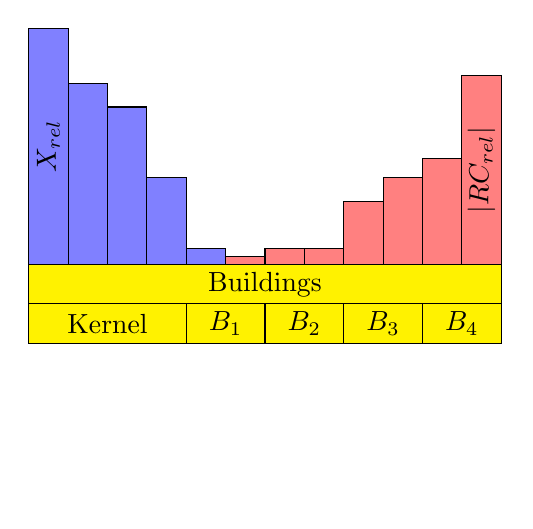
\begin{tikzpicture}
%		\draw[help lines] (0,0) grid (6,4);
		\fill[white] (0, -2) rectangle ++(6,0.5);		
		\draw[fill=yellow] (0, 0.5) rectangle ++(6,0.5) node[pos=.5] {Buildings};		
		\draw[fill=yellow] (0, 0) rectangle ++(2,0.5) node[pos=.5] {Kernel};
		\draw[fill=yellow] (2, 0) rectangle ++(1,0.5) node[pos=.5] {\(B_1\)};
		\draw[fill=yellow] (3, 0) rectangle ++(1,0.5) node[pos=.5] {\(B_2\)};
		\draw[fill=yellow] (4, 0) rectangle ++(1,0.5) node[pos=.5] {\(B_3\)};		\draw[fill=yellow] (5, 0) rectangle ++(1,0.5) node[pos=.5] {\(B_4\)};
		
		\draw[fill=blue!50] (0, 1) rectangle ++(0.5,3) node[pos=.5, rotate=90] {\(X_{rel}\)};
		\draw[fill=blue!50] (0.5, 1) rectangle ++(0.5,2.3);
		\draw[fill=blue!50] (1, 1) rectangle ++(0.5,2);
		\draw[fill=blue!50] (1.5, 1) rectangle ++(0.5,1.1);
		\draw[fill=blue!50] (2, 1) rectangle ++(0.5,0.2);
		
		\draw[fill=red!50] (2.5, 1) rectangle ++(0.5,0.1);
		\draw[fill=red!50] (3, 1) rectangle ++(0.5,0.2);
		\draw[fill=red!50] (3.5, 1) rectangle ++(0.5,0.2);
		\draw[fill=red!50] (4, 1) rectangle ++(0.5,0.8);
		\draw[fill=red!50] (4.5, 1) rectangle ++(0.5,1.1);
		\draw[fill=red!50] (5, 1) rectangle ++(0.5,1.35);
		\draw[fill=red!50] (5.5, 1) rectangle ++(0.5,2.4) node[pos=.5, rotate=90] {\(|RC_{rel}|\)};
	\end{tikzpicture}
	\caption{Standard sorting method for kernel search\cite{angelelli2010kernel}: Selection variables are sorted globally by their relaxed value (decreasing) at optimum and by their absolute reduced costs (increasing).}\label{fig:kernel-std-sort}
\end{figure}

\begin{figure}
	\centering
	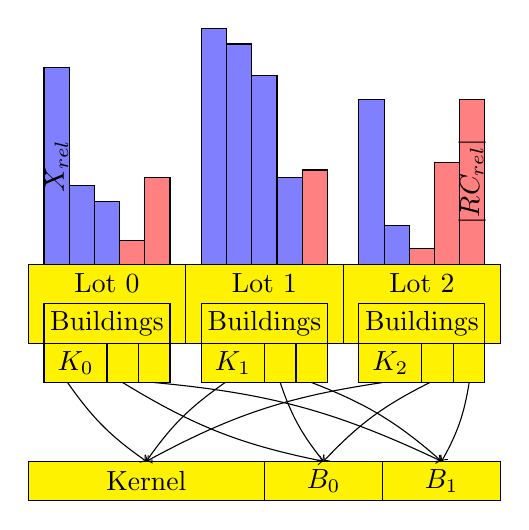
\begin{tikzpicture}
		\draw[fill=yellow] (0, 0) rectangle ++(2,1) node[pos=.5, yshift=7.5] {Lot 0};
		\draw[fill=yellow] (2, 0) rectangle ++(2,1) node[pos=.5, yshift=7.5] {Lot 1};
		\draw[fill=yellow] (4, 0) rectangle ++(2,1) node[pos=.5, yshift=7.5] {Lot 2};
		\draw[fill=yellow] (0.2, 0) rectangle ++(1.6,0.5) node[pos=.5] {Buildings};
		\draw[fill=yellow] (2.2, 0) rectangle ++(1.6,0.5) node[pos=.5] {Buildings};
		\draw[fill=yellow] (4.2, 0) rectangle ++(1.6,0.5) node[pos=.5] {Buildings};
		
		\draw[fill=blue!50] (0.2, 1) rectangle ++(0.32,2.5) node[pos=.5, rotate=90] {\(X_{rel}\)};
		\draw[fill=blue!50] (0.52, 1) rectangle ++(0.32,1);
		\draw[fill=blue!50] (0.84, 1) rectangle ++(0.32,0.8);
		\draw[fill=red!50] (1.16, 1) rectangle ++(0.32,0.3);
		\draw[fill=red!50] (1.48, 1) rectangle ++(0.32,1.1);
		
		\draw[fill=blue!50] (2.2, 1) rectangle ++(0.32,3);
		\draw[fill=blue!50] (2.52, 1) rectangle ++(0.32,2.8);
		\draw[fill=blue!50] (2.84, 1) rectangle ++(0.32,2.4);
		\draw[fill=blue!50] (3.16, 1) rectangle ++(0.32,1.1);
		\draw[fill=red!50] (3.48, 1) rectangle ++(0.32,1.2);
		
		\draw[fill=blue!50] (4.2, 1) rectangle ++(0.32,2.1);
		\draw[fill=blue!50] (4.52, 1) rectangle ++(0.32,0.5);
		\draw[fill=red!50] (4.84, 1) rectangle ++(0.32,0.2);
		\draw[fill=red!50] (5.16, 1) rectangle ++(0.32,1.3);
		\draw[fill=red!50] (5.48, 1) rectangle ++(0.32,2.1) node[pos=.5, rotate=90] {\(|RC_{rel}|\)};
		
		\draw[fill=yellow] (0.2, -0.5) rectangle ++(0.8,0.5) node[pos=.5] {\(K_0\)};
		\draw[fill=yellow] (1, -0.5) rectangle ++(0.4,0.5);
		\draw[fill=yellow] (1.4, -0.5) rectangle ++(0.4,0.5);
		
		\draw[fill=yellow] (2.2, -0.5) rectangle ++(0.8,0.5) node[pos=.5] {\(K_1\)};
		\draw[fill=yellow] (3, -0.5) rectangle ++(0.4,0.5);
		\draw[fill=yellow] (3.4, -0.5) rectangle ++(0.4,0.5);
		
		\draw[fill=yellow] (4.2, -0.5) rectangle ++(0.8,0.5) node[pos=.5] {\(K_2\)};
		\draw[fill=yellow] (5, -0.5) rectangle ++(0.4,0.5);
		\draw[fill=yellow] (5.4, -0.5) rectangle ++(0.4,0.5);
		
		\draw[fill=yellow] (0, -2) rectangle ++(3,0.5) node[pos=.5] {Kernel};
		\draw[fill=yellow] (3, -2) rectangle ++(1.5,0.5) node[pos=.5] {\(B_0\)};
		\draw[fill=yellow] (4.5, -2) rectangle ++(1.5,0.5) node[pos=.5] {\(B_1\)};
		
		\draw[->] (0.5, -0.5) to [bend right=10] (1.5, -1.5);
		\draw[->] (2.5, -0.5) to [bend right=10] (1.5, -1.5);
		\draw[->] (4.5, -0.5) to [bend right=10] (1.5, -1.5);
		\draw[->] (1.2, -0.5) to [bend right=10] (3.75, -1.5);
		\draw[->] (3.2, -0.5) to [bend right=10] (3.75, -1.5);
		\draw[->] (5.1, -0.5) to [bend right=10] (3.75, -1.5);
		\draw[->] (1.6, -0.5) to [bend left=10] (5.25, -1.5);
		\draw[->] (3.6, -0.5) to [bend left=10] (5.25, -1.5);
		\draw[->] (5.6, -0.5) to [bend left=10] (5.25, -1.5);
	\end{tikzpicture}
	\caption{Sorting method utilized for this project}\label{fig:kernel-cust-sort}
\end{figure}

Instead of a global sorting method as depicted in \cref{fig:kernel-std-sort}, where the LP relaxation is resolved and the variables are then ordered by decreasing relaxed value and by increasing reduced cost, a different approach has been choosen: the kernel and the buckets are constructed by selecting sub-kernels and sub-buckets from each different lot. Lots selection is then left for decision to Gurobi during the solution of the sub problem. We then treat each lot buildings as a single instance to be ordered through the method depicted in \cref{fig:kernel-std-sort}. A visual representation of this sorting method is depicted in \cref{fig:kernel-cust-sort}. 

Given a set of lots \(\mathbf{I} = \big\{1...\bar{n}\}\) each containing \(n_i\) buildings, the list of buildings in each lot \(\mathbf{C}\), and the sizes of the sub-kernels and sub-buckets, the sorting algorithm works as described in \cref{alg:kernel-sort-cust}.

\begin{algorithm}
	\caption{Kernel Search sorting algorithm used}\label{alg:kernel-sort-cust}
	\begin{algorithmic}
		\Function{SortBuildings}{$\mathbf{I}$, $\mathbf{C}$, $K_{size}$, $B_{size}$}
			\State $rel \gets$ \Call{ResolveLPRelaxation}{$\mathbf{I}$}
			\State $K \gets \emptyset$
			\State $B \gets \emptyset$
			\ForAll{$l \in \mathbf{I}$}
				\State \Call{SortLot}{$l$, $rel$}
				\State $K \gets K \cup $\Call{GetBuildings}{$l$, $0$, $K_{size}$}
				\State $len \gets K_{size}$
				\State $i \gets 0$
				\While{$len \leq |C_i|$}
					\State $B[i] = B[i] \cup$\Call{GetBuildings}{$l$, $len$, $B_{size}$}
					\State $len \gets len + B_{size}$
					\State $i \gets i + 1$
				\EndWhile
			\EndFor
			\State \Return{K, B}
		\EndFunction
	\end{algorithmic}
\end{algorithm}

The concept behind \cref{alg:kernel-sort-cust} is the following: after having solved the LP relaxation of the main problem, each lot can be seen as a \ac{MKP} with additional global constraints. Because of this, each lot of buildings can now be sorted as if it was a simpler problem as described by E.Angelelli et al.\cite{angelelli2010kernel} by sorting the variables by value and reduced costs. 
We can then identify a kernel \(K_l\) for each lot \(l \in \textbf{I}\) as the \(K_{size}\) most promising buildings for the lot. We define the problem's kernel \(K\) as the union of each sub-kernel \(K_l\). Formally: \[K = \bigcup_{l \in \mathbf{I}} K_l\]

During the kernel search iteration procedure, multiple sub-problems have to be solved with the addition of new variables added to the problem in the form of buckets. We decided to iterate over each bucket of fixed size \(|\mathbf{I}| \cdot B_{size}\) composed similarly to the kernel \(K\) as following: \[B_i = \bigcup_{l \in \mathbf{I}} B_li\]

Each time a new bucket is added, a new constraint, defined in \cref{eqn:must-select} is added to the problem stating that at least one building of the newly added bucket \(B_i\) has to be choosen in a new incumbent solution for the current iteration. Also, once a new incumbent solution has been found, a new cutoff constraint must be added excluding all solutions with objective value lower than or equal to the newly found incumbent soluton.

\begin{equation}\label{eqn:must-select}
	\sum_{i \in \mathbf{I}, j \in C_i : x_{ij} \in B_i} x_{ij} \geq 1 
\end{equation}

On new solutions, the variables chosen in the last bucket are then included in the kernel set \(K\).

Ideally, non-useful lots are going to be excluded in the first few iterations and thus not providing kernel set additions reducing the number of variables in the problem. Contrarily, useful lots may be excluded in the beginning limiting their ability to provide variables and so to be selected again. This problem can be managed by applying the solution defined in \cref{sec:lot-iteration}.

\subsection{Lot iteration}\label{sec:lot-iteration}
In order not to reject useful lots and to allow for faster sub-problems, we managed to implement a lot-based iteration step. The algorithm becomes effectively a kernel search made amongst buildings inside a kernel search made amongst lots.

This method allows to reiterate over bucket inside the most promising lots and still add new variables to the problem.

The conceptual algorithm is reported in \cref{alg:lot-iter}. The idea of the algorithm is to reduce the initial number of variables in the kernel and the buckets by forcing part of the \(y_i\) variables to zero. The sub-problem is solved with the kernel search heuristic discussed in \cref{sec:heuristic}. After this preliminary solution, the another set of \(y_i\) variables is allowed to be choosen and the iteration repeated by keeping the initial kernel. This allows to reintroduce discarded bucket variables from the previous iteration in the previous lot set and still extend the kernel set with the new lot's variables. Lot sorting is discussed in \cref{sec:lot-iteration-ordering}

\begin{algorithm}
	\caption{Lot iteration algorithm}\label{alg:lot-iter}
	\begin{algorithmic}
		\Function{IterateLots}{$\mathbf{I}$, $\mathbf{C}$, $K_{size}$, $B_{size}$}
		\State $curLots \gets \emptyset$
		\State $sol \gets \emptyset$
		\State \Call{SortLots}{$\mathbf{I}$, $\mathbf{C}$}
		\While{$I \neq \emptyset$}
			\State $curLots \gets curLots \cup $\Call{GetFirstN}{$I$}
			\State $I \gets I - curLots$
			\State $sol \gets $\Call{BuildingsKernelSearch}{$curLots$, $\mathbf{C}$, $K_{size}$, $B_{size}$, $sol$}
		\EndWhile
		\State \Return $sol$
		\EndFunction
	\end{algorithmic}
\end{algorithm}

\subsubsection{Lot ordering}\label{sec:lot-iteration-ordering}
Given a set of lots \(\mathbf{I}\) and the current incumbent solution \(\bar{S}\), for each lot \(l \in \mathbf{I}: S(y_l) = 0\) we define the \(l\)-relaxation over the solution \(\bar{S}\) as a \ac{MKP} with the buildings of lot \(l\) constraining all its local capacity constraints and all global constraints in a reduced form \(\bar{R}\). 

The reduced form of the global constraints \(\bar{R}\) is calculated as \[\bar{R}_i = R_i - \sum_{j \in C_l} a^r_{lj}x_{lj} \]

The LP relaxation optimal objective value is then taken as a metric for sorting of the lots.



\subsubsection{Kernel Filtering}\label{sec:kernel-filterung}

\clearpage
\printbibliography

\end{document}